\section{Induzione elettromanietica}
\subsection{Forza elettromotrice(f.e.m.)}
La fem si misura in Volt e fornisce energia ai portaotri di cariche
per permettere il flusso di corrente.

\subsection{Induzione elettromanietica}
\begin{figure}[H]
    \centering
    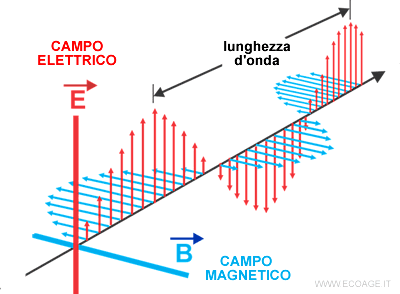
\includegraphics[width=0.3\linewidth]{imgs/17 - induzione elettromanietica.png}
    \label{fig:induzione_elettromanietica}
    \caption{Comportamento campo elettrico e magnetico}
\end{figure}
Ogni variazione del campo magnetico, provoca un campo elettrico.

\subsection{Legge di induzione elettromanietica}
La corrente indotta viene generata quando un campo magnetico varia.

\subsection{Legge di Faraday}
La fem indotta dipende dalla velocità di cariazione del flusso magnetico:
\begin{equation*}
    \epsilon = -\frac{d\phi_B}{dt}
\end{equation*}

La legge di faraday associa $1V = 1\frac{Wb}{s}$.
Se una bobina è fatta da più spire, usiamo la regola con La
concatenzaione:
\begin{equation}
    \epsilon_T = N\epsilon = N\Biggl(-\frac{d\phi_B}{dt}\Biggr)
\end{equation}

\subsection{Legge di Lenz}
Per capire il segno della fem indotta, bisogna usare Lenz.
Il senso della corrente indotta è tale che il suo contributo
al campo magnetico si oppone alla variazione del flusso magnetico
che produce la corrente indotta stessa.

Per effettuare il calcolo, bisogna definire il verso dei vettori
delta sperficie.


%TODO: Sistemare la legge di lenz perche è una merda e non volgio farla

\subsection{F.e.m. di movimento}

\begin{figure}[H]
    \centering
    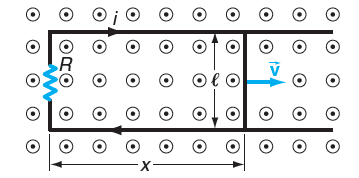
\includegraphics[width=0.4\linewidth]{imgs/18 fem indotta.png}
    \label{fig:fem_movimento}
    \caption{Fem indotta dal movimento}
\end{figure}
Il campo di induzione magnetica del circuito(perpendicolare al piano),
è:
\begin{equation}
    \phi_B = \iint{\vec{B}\cdot d\vec{S}} = Blx\cos\theta
\end{equation}

dove la $l$ e la $x$ sono l'area del circuito considerato in quel momento.

Visto che il filo scorre, l'area cambia, quindi il flusso cambia.
\begin{equation}
    \frac{d\phi_B}{dt} = \frac{d(Blx)}{dt} = Blv\cos\theta
\end{equation}
dove $v$ è la velocità(spazio fratto tempo:)).

Quindi la legge di faraday dice che la fem indotta nel circuito è:
\begin{equation}
    \epsilon = Blv\cos\theta
\end{equation}

\subsection{Campi elettrici indotti}
Se un conduttore si muove in un campo di induzione magnetica
uniforme, i portatori di carica si muoveranno con velocità
media $\vec{v}$.

La forza elettrica e magnetica agente sulle particelle è:
\begin{equation}
    \vec{F} = q(\vec{E}+\vec{v}\times\vec{B})
\end{equation}

Gli esperimenti confermano che il campo elettrico E esercita
una forza F sulla qualunque carica q presente nella regione.
La fem indotta è (più o meno) il lavoro per unità di carica
compiuto dalla forza elettrica.
\begin{equation}
    \epsilon = \frac{W}{q} = \oint{\vec{E}\cdot d\vec{l}}
\end{equation}

\subsection{Campo elettrico indotto Vs elettrostatico}
Campo elettrostatico(prodotto da una distribuzione di cariche con coulomb)
differisce dal campo elettrico indotto per:
\begin{itemize}
    \item $\oint{\vec{E}\cdot d\vec{l}} = 0$ per campo elettrostatico
    \item $\oint{\vec{E}\cdot d\vec{l}} = \epsilon$ nel campo indotto
\end{itemize}


Il campo elettrico indotto è non conservativo e viene prodotto
da un campo magnetico variabile.

\subsection{Legge di Faraday: forma integrale}
La legge di Faraday espressa in termini dei Campi è valida 
solo in presenza di conduttori, sennò cade il principio della fem.
La forma integrale(o legge generale) è:
\begin{equation}
    \oint{\vec{E}\cdot d\vec{l}} = 
    -\frac{d}{dt}\iint{\vec{B}\cdot d\vec{S}}
\end{equation}

